%\documentclass[PhD,two side]{srmuthesis}
%\documentclass[MS]{srmuthesis}
%\documentclass[MTech]{srmuthesis}
\documentclass[BTech]{srmuthesis}
\usepackage{times}
\usepackage{t1enc}
\usepackage{tikz}
\usepackage{subfigure}
\usepackage{pgfplots}
\usepackage{setspace} 
\usepackage{geometry}
\usepackage{graphicx}
\usepackage{epstopdf}
\usepackage{lscape}
\usepackage{fancyhdr}
\usepackage{natbib}
\usepackage{hyperref} % hyperlinks for references.
\usepackage{amsmath} % easier math formulae, align, subequations \ldots
\usepackage{amssymb}
\usepackage{wasysym}
\usepackage{titlesec}
\usepackage{textcomp}
\usepackage{pifont}
\usepackage{appendix} 
\usetikzlibrary{decorations.pathmorphing}
\usetikzlibrary{shapes,arrows,shadows,patterns}
\usepackage[printonlyused]{acronym}
%\usepackage{nomencl}
%\newcommand{\bigsize}{\fontsize{16pt}{20pt}\selectfont}
%\renewcommand\nomname{\centerline {NOTATION}}
%\makenomenclature
\setcounter{MaxMatrixCols}{20}
\captionsetup[figure]{labelfont=bf}
\begin{document}
%%%%%%%%%%%%%%%%%%%%%%%%%%%%%%%%%%%%%%%%%%%%%%%%%%%%%%%%%%%%%%%%%%%%%%
% Title page

\title{MULTIPLE IMAGE COMPRESSION} % Enter The Project Title

\firstauthor{ SANJAY KV }% Enter The Student name
\firstauthorregno{[Reg No: RA1411003020012]}
\secondauthor{ ANANTHU PRESANTH }% Enter The Student name
\secondauthorregno{[Reg No: RA1411003020024]}
\thirdauthor{ PADBANABHAN ELANGOVAN } % If there is no third author, leave the space blank like \thirdauthor{}
\thirdauthorregno{[Reg No: RA1411003020024]}

\guide{Mr.ARUN KUMAR} % Enter your guide's name
\designation{Professor} % Enter your guide's designation
\guidedepartment{Computer Sciene \& Engineering} % Enter the department name of your Guide 
\hod{Dr.  J.JAGADEESAN,M.Tech.,Ph.D.,  } % Enter HOD's name
\department{Computer Science and Engineering} % Enter your department name
\date{APRIL 2017} % Enter month and year of submission
%\nocite{*}

\maketitle
%%%%%%%%%%%%%%%%%%%%%%%%%%%%%%%%%%%%%%%%%%%%%%%%%%%%%%%%%%%%%%%%%%%%%%
%\vspace*{3in}
%\begin{center}
%{\Huge Dedicated to my Parents}
%\end{center}
%%%%%%%%%%%%%%%%%%%%%%%%%%%%%%%%%%%%%%%%%%%%%%%%%%%%%%%%%%%%%%%%%%%%%%
% Certificate
\certificate
%\vspace*{0.5in}



%%%%%%%%%%%%%%%%%%%%%%%%%%%%%%%%%%%%%%%%%%%%%%%%%%%%%%%%%%%%%%%%%%%%%%
% Abstract

\abstract
\begin{doublespacing}
{\large\noindent The world is Digitizing day by day, so the expectations for highest Quality contents in budget range is increasing. So Technique such as Image Compression System is Relevant.
The research area of image compression provides many widely-used compression methods that provide relevant back-ground and a basis of comparison for our application.
Image compression schemes can be divided into two categories:
•	Lossless compression and
•	Lossy compression.
Lossless compression allows the exact input signal to be reconstructed after it is compressed.
Lossy Image compression reduces the image fidelity, when an image is compressed at low bitrates. Thereby reduction in Quality is seen


\end{doublespacing}

\pagebreak
%%%%%%%%%%%%%%%%%%%%%%%%%%%%%%%%%%%%%%%%%%%%%%%%%%%%%%%%%%%%%%%%%%%%%%
% Acknowledgements
\acknowledgements
I would like to express my deepest gratitude to my guide, Mr.Arun Kumar 
his valuable guidance, consistent encouragement, personal caring, timely help and providing me with an excellent atmosphere for doing research. All through the work, in spite of his busy schedule, he has extended cheerful and cordial support to me for completing this research work.\\



\begin{flushright}
{\bf SANJAY KV}\\
{\bf ANANTHU PRESANTH }\\
{\bf PADBANBHAN ELANGOVAN}

\end{flushright}
%%%%%%%%%%%%%%%%%%%%%%%%%%%%%%%%%%%%%%%%%%%%%%%%%%%%%%%%%%%%%%%%%
% Table of contents etc.

\begin{singlespace}
\tableofcontents
\thispagestyle{empty}

\listoftables
\addcontentsline{toc}{chapter}{LIST OF TABLES}
\listoffigures
\addcontentsline{toc}{chapter}{LIST OF FIGURES}
\end{singlespace}


%%%%%%%%%%%%%%%%%%%%%%%%%%%%%%%%%%%%%%%%%%%%%%%%%%%%%%%%%%%%%%%%%%%%%%
\abbreviations
%\begin{acronym}[longest acronym must be entered here]
\begin{acronym}[OKID/ERA]

%\acro{acronym}{in detail}
\acro{ABC}{Artificial Bee Colony}
\acro{ACO}{Ant Colony Optimization}
\acro{BA}{Bees Algorithm}
\acro{BFO}{Bacterial Foraging Optimization}
\acro{BM} {Bending Moment}
\acro{CMIR}{Condensed Model Identification and Recovery}
\acro{CMTM}{Consistent Mass Transfer Matrix}
\acro{CPU}{Central Processing Unit}
\acro{CS}{Cuckoo Search}
\acro{CSI}{Complete Structural Identification}
\acro{DAQ}{Data Acquisition}
\acro{DOF}{Degrees Of Freedom}
\acro{DTM}{Damped Transfer Matrix}
\acro{EA}{Evolutionary Algorithm}
\acro{EKF}{Extended Kalman Filter}
\acro{ERA}{Eigen system Realization Algorithm}
\acro{FE}{Finite Element}
\acro{FRF}{Frequency Response Function}
\acro{GA}{Genetic Algorithm}
\acro{LCTM}{Lumped Crack Transfer Matrix}
\acro{LM}{Levenberg-Marquardt}
\acro{LMTM}{Lumped Mass Transfer Matrix}
\acro{LS}{Least Square}
\acro{MAE}{Mean Absolute Error}
\acro{MSE}{Mean Square Error}
\acro{MSI}{Modular Smart Interface}
\acro{OKID/ERA}{Observer Kalman Filter Identification/Eigen Realization Algorithm}
\acro{PSO}{ Particle Swarm Optimization}
\acro{SA}{Simulated Annealing}
\acro{SCTM}{Single Crack Transfer Matrix}
\acro{SF} {Shear Force}
\acro{SHM}{Structural Health Monitoring}
\acro{SI}{Structural Identification}
\acro{SS}{Sub-Structure}
\acro{SSI}{Sub-Structural Identification}
\acro{TCTM}{Two Crack Transfer Matrix}
\acro{TM}{Transfer Matrix}
\end{acronym}
% Use the syntax \ac{acronym} whereever you use this acronym.
% Abbreviations

%\noindent 
%\begin{tabbing}
%xxxxxxxxxxx \= xxxxxxxxxxxxxxxxxxxxxxxxxxxxxxxxxxxxxxxxxxxxxxxx \kill
%\textbf{TM}   \> Transfer Matrix \\
%\textbf{LMTM} \> Lumped Mass Transfer matrix \\
%\textbf{CMTM} \> Consistent Mass Transfer matrix \\
%\textbf{SCTM} \> Single Crack Transfer matrix \\
%\textbf{LCTM} \> Lumped Crack Transfer matrix \\
%\textbf{DCTM} \> Double Crack Transfer matrix \\
%\textbf{DOF} \> Degrees Of Freedom \\
%\textbf{GA} \> Genetic Algorithm  \\
%\textbf{PSO} \> Particle Swarm Optimization \\
%\textbf{SI} \> Structural Identification \\
%\end{tabbing}

\pagebreak

%%%%%%%%%%%%%%%%%%%%%%%%%%%%%%%%%%%%%%%%%%%%%%%%%%%%%%%%%%%%%%%%%%%%%%
% Enter the symbols used in the thesis in alphabatical order
\chapter*{\centerline{LIST OF SYMBOLS}}
\addcontentsline{toc}{chapter}{LIST OF SYMBOLS}
%\nomenclature{b}{Width of the beam}
%\nomenclature{r}{Number of DOF}
%\nomenclature{n}{Number of elements}
%\nomenclature{h}{Thickness of the beam}
%\nomenclature{$\theta$}{Length of the beam}
%\nomenclature{$\omega$}{Circular frequency}
\begin{doublespace}
\begin{tabbing}
%\printnomenclature
xxxxxxxxxxx \= xxxxxxxxxxxxxxxxxxxxxxxxxxxxxxxxxxxxxxxxxxxxxxxx \kill
\textbf{$\alpha$, $\beta$}   \> Damping constants  \\
\textbf{$\theta$}   \> Angle of twist, rad  \\
\textbf{$\omega$}   \> Angular velocity, rad/s  \\
\textbf{$b$}   \> Width of the beam,  m \\
\textbf{$h$}   \> Height of the beam,  m \\
\textbf{$\{f(t)\}$}   \> force vector  \\
\textbf{$[K^e]$}  \> Element stiffness matrix\\
\textbf{$[M^e]$}  \> Element mass matrix \\
\textbf{$\{q(t)\}$}   \> Displacement vector  \\
\textbf{$\{\dot{q}(t)\}$}   \> Velocity vector  \\
\textbf{$\{\ddot{q}(t)\}$}   \> Acceleration vector  \\


\end{tabbing}
\end{doublespace}

\pagebreak
\clearpage
% The main text will follow from this point so set the page numbering
% to arabic from here on.
\pagenumbering{arabic}


%%%%%%%%%%%%%%%%%%%%%%%%%%%%%%%%%%%%%%%%%%%%%%%%%%
% Introduction.

%Enter your chapter number here
\chapter{INTRODUCTION}
\label{chap:intro}
\section{Overview}
 \ac{SI} is typically an inverse process whereby structural parameters such as stiffness, damping properties are identified from input excitation and output responses.
 

 Generally, Engineering problems can be classified into forward and inverse problems \citep{ssikoh}. In forward problems, the system output responses are calculated from the known system properties and input responses as shown in Figure \ref{fig:fp} whereas in inverse problems, the system parameters are identified based on the input and output responses of the system which is shown in Figure \ref{fig:ip}. 
 \begin{figure}[htpb]
  \centering
    \tikzstyle{block} = [rectangle, line width=0.75pt,draw,  text width=20mm, text centered,  minimum height=10mm]
    \tikzstyle{line} = [draw, line width=0.75pt, -latex']
   \begin{tikzpicture}
  \node [block,text width=30mm] (input) {\bf\footnotesize Input Excitation};
  \node [block,right of=input,text width=35mm,node distance = 45mm] (nummode) {\bf \footnotesize Numerical model};
   \node [block, above of=nummode,text width=35mm,node distance = 20mm] (para) {\bf \footnotesize System Parameters (Mass, Stiffness and Damping co-efficient)};
  \node [block,right of=nummode,text width=35mm,node distance = 45mm] (output) {\bf \footnotesize Output Responses (Acceleration, Velocity and Displacement)};
  % Draw edges
        \path [line] (input) -- (nummode);
        \path [line] (para) -- (nummode);
         \path [line] (nummode) -- (output);
 \end{tikzpicture}
 \caption{Forward problem}
 \label{fig:fp}
 \end{figure}
 \begin{figure}[htpb]
   \centering
     \tikzstyle{block} = [rectangle, line width=0.75pt,draw,  text width=20mm, text centered,  minimum height=10mm]
     \tikzstyle{line} = [draw, line width=0.75pt, -latex']
    \begin{tikzpicture}
   \node [block,text width=30mm] (input) {\bf\footnotesize Input Excitation};
   \node [block,right of=input,text width=35mm,node distance = 45mm] (nummode) {\bf \footnotesize Numerical model};
    \node [block, right of=nummode,text width=35mm,node distance = 45mm] (para) {\bf \footnotesize System Parameters (Mass, Stiffness and Damping co-efficient)};
   \node [block,above of=nummode,text width=35mm,node distance = 20mm] (output) {\bf \footnotesize Output Responses (Acceleration, Velocity and Displacement)};
   % Draw edges
         \path [line] (input) -- (nummode);
         \path [line] (output) -- (nummode);
          \path [line] (nummode) -- (para);
  \end{tikzpicture}
  \caption{Inverse problem}
  \label{fig:ip}
  \end{figure}
  For a structure, the input excitation is a periodic force and the output responses are displacement, velocity and acceleration. The input force can be measured using force transducer and the output responses can be measured respectively using vibration pick-ups, velometer and accelerometer. Some \ac{SI} algorithms require measurement of all responses or any one of the output responses. Since the input and output responses are measurable for a structure with unknown parameters, the \ac{SI} problem is an inverse problem which identifies structural or damage parameters.\\ \vspace{-5mm}
  \subsection{Sub sections} 
  Sub-sections must be numbered as shown in this text. 
  \subsubsection{Sub-sub sections}
  Sub-sections of sub section are not to be numbered and it should be in bold as shown in this text. 
 \chapter{LITERATURE SURVEY}


\section{Image Compression Survey}
\citet{george} showed that the magnitude of change in natural frequencies is a function of the severity and of the location of deterioration in structures. The modal analysis has been carried out on a welded steel frame and a wire rope with damage. \citet{gredia} proposed a direct method for determining six flexural stiffnesses of a thin anisotropic plate. In this method, natural frequencies \citep{Leo} and mode shapes have been processed using \ac{LS} technique.


\chapter{System Analysis}
All the symbols used in the text must be listed out in the list of symbols page in alphabetic order, and explained with units. Equations must be written with central alignment and numbered with section number . equation number. 
\begin{equation}
[M^e]\{\ddot{q}(t)\}+[C^e]\{\dot{q}(t)\}+[K^e]\{q(t)\}=\{f(t)\}
\label{eq:mkceqn}
\end{equation}  
the element stiffness matrix is
\begin{equation}
[K^e]=\frac{EI}{l_e^3}\begin{bmatrix}
12&6l_e &-12&6l_e\\
6l_e&4l_e^2&-6l_e&2l_e^2\\
-12&-6l_e&12&-6l_e\\
6l_e&2l_e^2&-6l_e&4l_e^2
\end{bmatrix}
\label{eq:sm}
\end{equation}
and the element consistent mass matrix is
\begin{equation}
[M^e]=\frac{\rho Al_e}{420}\begin{pmatrix}
156&22l_e &54&-13l_e\\
22l_e&4l_e^2&13l_e&-3l_e^2\\
54&13l_e&156&-22l_e\\
-13l_e&-3l_e^2&-22l_e&4l_e^2
\end{pmatrix}
\label{eq:cmm}
\end{equation}
\begin{equation}
[C]=\alpha[M]+\beta[K]
\end{equation}
A matrix equation with square matrices and vectors,
\begin{equation}
\begin{Bmatrix}
-M_1(t)\\
-V_1(t)\\
M_2(t)\\
V_2(t)\end{Bmatrix}=\begin{bmatrix}
D_{11}&D_{12}&D_{13}&D_{14}\\
D_{21}&D_{22}&D_{23}&D_{24}\\
D_{31}&D_{32}&D_{33}&D_{34}\\
D_{41}&D_{42}&D_{43}&D_{44}\end{bmatrix}\begin{Bmatrix}
v_1(t)\\
\theta_1(t)\\
v_2(t)\\
\theta_2(t)\end{Bmatrix}
\label{eq:D}
\end{equation}
\chapter{System Design}
\section{Tables and Figures} 
 By the word Table, is meant tabulated numerical data in the body of the project report as well as in the appendices. All other non-verbal materials used in the body of the project work and appendices such as charts, graphs, maps, photographs and diagrams may be designated as figures\footnote{type footnote here}.
  The format for tables  is given below. The table must referred in the text as Table. (\ref{tab:frmcl}). The title of the table with table number should be written at the top of the table with center aligned as shown below.\footnote{An example footnote.}.
 \begin{table}[htpb]
      \centering
      \caption{Error in identified parameters}
      \begin{tabular}{|c|c|c|c|c|c|}
      	\hline
      	\multicolumn{2}{|c|}{Exact parameter} &               \multicolumn{4}{c|}{Identified crack location (\% of error)}               \\ \cline{3-6}
      	\multicolumn{2}{|c|}{}                & \multicolumn{2}{c|}{Complete measurement} & \multicolumn{2}{|c|}{Incomplete measurement} \\ \hline
      	Depth($\xi$) &  Location($\lambda$)   &  Noise free   &         5\% Noise         &  Noise free   &          5\% Noise           \\ \hline
      	   0.067     &          0.5           & 0.501(0.2\%)  &       0.503(0.6\%)        & 0.501(0.2\%)  &        0.496(-0.8\%)         \\
      	    0.50     &          0.5           & 0.498(-0.4\%) &       0.506(1.2\%)        & 0.498(-0.4\%) &         0.508(1.6\%)         \\ \hline
      \end{tabular}
        \label{tab:frmcl}
      \end{table}\\
      
    Figures must be drawn at the appropriate places and must be referred in the same page in the text. Figures should be referred in the text as Figure \ref{fig:beam}. 
      \begin{figure}[htpb]
      \centering
      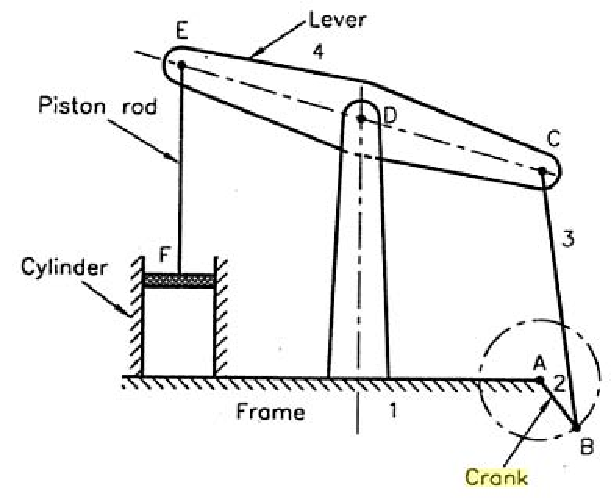
\includegraphics[scale=0.5]{beam_engine.pdf}
      \caption{\bf Beam engine}
      \label{fig:beam}
      \end{figure}
      Title of figures must be center aligned and should be displayed at the bottom of the figure as shown. \\
      
    \begin{figure}[htpb]
    \centering
    \subfigure[Elliptical trammel]{
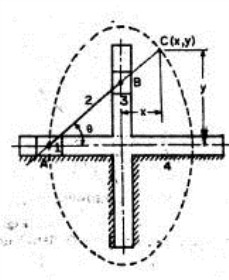
\includegraphics[scale=0.75]{ellipse.jpg}
\label{fig:ellipse}} \hspace{10mm}
\subfigure[Scotch Yoke]{
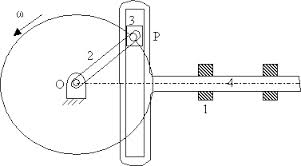
\includegraphics[scale=0.75]{scotch.jpg}
\label{fig:scotch}}
\caption{\bf Inversions of double slider crank chain}
\label{fig:4s}
    \end{figure}
     Multiple figures with same caption can be arranged as shown in Figure \ref{fig:4s} and they are referred in text such as Figure \ref{fig:ellipse} and Figure \ref{fig:scotch}. The graphs should be drawn at appropriate places with center alignment and it should be referred in text. \\
     \begin{figure}[htpb]
     \centering
     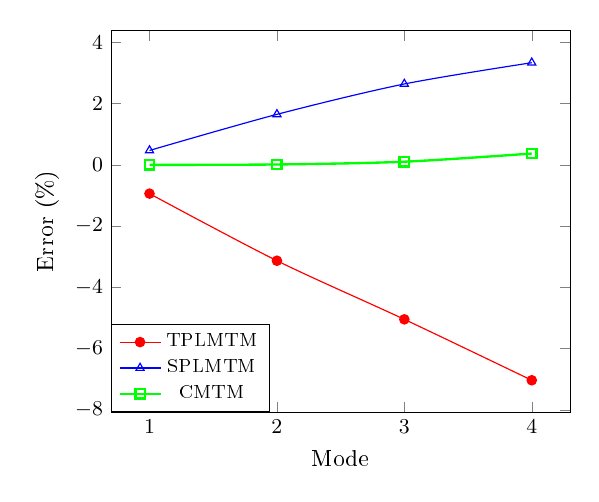
\begin{tikzpicture}[scale=0.85]
         \begin{axis}[
             xlabel=Mode,
             ylabel= Error (\%), tick label style={font=\small}, xtick={1,2,3,4},legend style={font=\footnotesize,at={(0,0)},anchor=south west}]
         \addplot[smooth,line width=0.5pt,mark=*,color=red] 
         plot coordinates {
             (1,-0.939212)
             (2,-3.130594064)
             (3,-5.044603033)
             (4,-7.033277189)
         };
         \addplot[smooth, line width=0.5pt,mark=triangle,color=blue]
             plot coordinates {
                 (1,0.46960605)
                 (2,1.648557512)
                 (3,2.640499554)
                 (4,3.334547275)
             };
          \addplot[smooth,line width=1pt,mark=square, color=green]
                 plot coordinates {
                     (1,0)
                     (2,0.012489072)
                     (3,0.102586976)
                     (4,0.369493634)
                 };
             \legend{TPLMTM\\SPLMTM\\CMTM\\}
         \end{axis}
         \end{tikzpicture}
         \caption{\bf Error in natural frequencies}
         \label{fig:natfrq}
         \end{figure}
         \chapter{Coding, Testing}
In this chapter, the program coding related to your work using MATLAB\texttrademark or C can be presented here. Numbered list can be typeset in LaTex as follows.
\begin{enumerate}
   \item  \textbf{Online LaTex editors} Such as \textbf{Share LaTex}, \textbf{Write LaTex}, \textbf{Papeeria} 
    are also available which do not require any installation. \vspace{5mm}
   \item  Documents can be typeset or edited in the online LaTex and output file can be down loaded.\vspace{5mm}
   \item  The LaTex template can generally be down loaded from the University/publisher's/ conference website. (.tex file) \vspace{5mm}
   \item Type the document in the respective template and run the program like C or MATLAB. \vspace{5mm}
   \item  The output document is formatted as .pdf or .ps and saved in the same file name and same folder. \vspace{5mm}
   \item  Some Standard LaTex templates are \textit{IEEE}, \underline{ASCE}, \textsf{ASME}, Elsevier etc. \vspace{5mm}
   \end{enumerate}
   Bullet points are generated in LaTex as follows:
   \begin{itemize}
          \item [\ding{92}] Requires installation of two packages.
     \item [\ding{92}]\textbf{MiKTeX} is a distribution of the typesetting system.
     \item [\ding{92}] MiKTeX provides the tools necessary to prepare documents using the TeX/LaTeX markup language. 
     \item [\ding{92}] \textbf{TeXstudio} is a cross-platform open source LaTeX editor with an interface. 
     \item [\ding{92}] Some other cross-platforms are Texmaker, Technic center, Winedt etc.,
     \item [\ding{92}] Install MiKTex first and TeXstudio at last.
      \end{itemize}
\chapter{Conclusion}
The Entire Project Document should have a \textbf{maximum of 80 Pages} (from cover to cover).\\
The Project Document along with Application Software should be submitted in a Soft Copy (CD )\\
\underline{\textbf{N.B.: Number of Copies to be submitted:}}
Guide - 1 hard copy, Department Library -1 hard copy \&
 Each Candidate -1 hard copy and Soft Copy (in CD)- 2 copies
\chapter{Future Enhancement}

%%%%%%%%%%%%%%%%%%%%%%%%%%%%%%%%%%%%%%%%%%%%%%%%%%%%%%%%%%%%
% Appendices.

\appendix
\chapter{VECTOR ALGEBRA}
\section{Product of Two Vectors}
\label{app:vp}
The product of two vectors are may be a scalar product or vector product. The scalar product of two vectors is also called as dot product. It is defined as $\vec{a} . \vec{b}=|\vec{a}||\vec{b}|cos\theta$ where $\theta$ is the angle between the two vectors $\vec{a}$ and $\vec{b}$\\

the cross product or vector product is a binary operation on two vectors in three-dimensional space and is denoted by the symbol $\times$. The cross product $\vec{a}\times\vec{b}$ of two linearly independent vectors $\vec{a}$ and $\vec{b}$ is a vector that is perpendicular to both and therefore normal to the plane containing them. 
\chapter{MATRIX ALGEBRA}
\section{Matrix Multiplication}
Matrix multiplication is a binary operation that takes a pair of matrices, and produces another matrix. Numbers such as the real or complex numbers can be multiplied according to elementary arithmetic. On the other hand, matrices are arrays of numbers, so there is no unique way to define multiplication of matrices. As such, in general the term ``matrix multiplication'' refers to a number of different ways to multiply matrices. 
%%%%%%%%%%%%%%%%%%%%%%%%%%%%%%%%%%%%%%%%%%%%%%%%%%%%%%%%%%%%
% Bibliography.

\begin{singlespace}
  \bibliography{thesis_refer} % Enter your .bib file name here
\end{singlespace}
%%%%%%%%%%%%%%%%%%%%%%%%%%%%%%%%%%%%%%%%%%%%%%%%%%%%%%%%%%%%
  \end{document}
